\documentclass[12pt,a4paper]{article}
\usepackage{graphicx}
\begin{document}
\begin{titlepage}
\title{Software Requirements Specification\\CS Marks System\\ \small Version: 3.0}
\date{\today}
\author{Neels van Rooyen u29052735\\
Luan van der Weshuizen u10134043\\
Ndivhuwo Nthambeleni u10001183\\
Cebolenkosi Makeleni u10534505\\
Dieter Doman u11002566\\
Christopher Crossman u10134842}
\maketitle
\end{titlepage}
\tableofcontents
\pagebreak
\section{Introduction}
\paragraph{}
The purpose of this document is to make an agreement between the developers and the client Mr Jan Kroeze from the Department of Computer Science about the requirements of the new Marks System that needs to be developed. This document is to ensure the scope of the project is correct and clear to all the stakeholders in this project. This document the basis for which further phases will be built on.
\section{Vision}
\paragraph{}
The purpose of the project is to develop a software solution which provides a web and mobile platform for markers, students and lecturers handle marks and marking in the Department of Computer Sciences. It will uphold the privacy of students so that students cannot see each others marks. It will reduce paper work and the chances that marks can be lost and provide a centralized repository for student marks. It will provide functionality to generate customizable reports at different levels of granularity.
\section{Background}
\paragraph{}
Currently a marker has to use paper in order to record, process and submit student marks. This process is lengthy and risky since marks get lost and people make mistakes adding up marks.
\section{The Stakeholders}
\subsection{The Client}
The Client is Mr Jan Kroeze at the Department of Computer Science.
\subsection{The Customers}
The Customers are the students of Computer Science modules as well as their markers and lecturers.
\subsection{Maintenance Users and Service Technicians}
The Project will be maintained by the departmental technical assistants in Tech-Team and Web-Team.
\section{Architecture requirements}
\subsection{Access Requirements}
\paragraph{}
The Project needs to be accessible from mobile devices, specifically Android devices, as well as Desktop web browsers.
\subsection{Quality Requirements}
\subsubsection{Performance}
\subsubsection{Computational Cost}
\subsubsection{Accessibility and Usability}
\subsubsection{Reliability}
\subsubsection{Security}
\subsubsection{Audit Requirements}
\subsubsection{Flexibility}
\subsubsection{Monitor Requirements}
\subsection{Integration Requirements}
\begin{itemize}
\item The Project must be integrated with the Computer Science web site.
\item Authentication must be done via LDAP.
\item Marks must be stored in Mysql
\end{itemize}
\subsection{Architecture Constraints}
\begin{itemize}
\item The Project needs to be created in the django framework.
\item The Project must be accessible from Android devices.
\end{itemize}
\section{Functional Requirements}
\subsection{Introduction}
\paragraph{}
This section discusses the application functionality required by the stakeholders.
\subsection{Scope and Limitations/Exclusions}
\subsubsection{High Level Use Case Diagram}
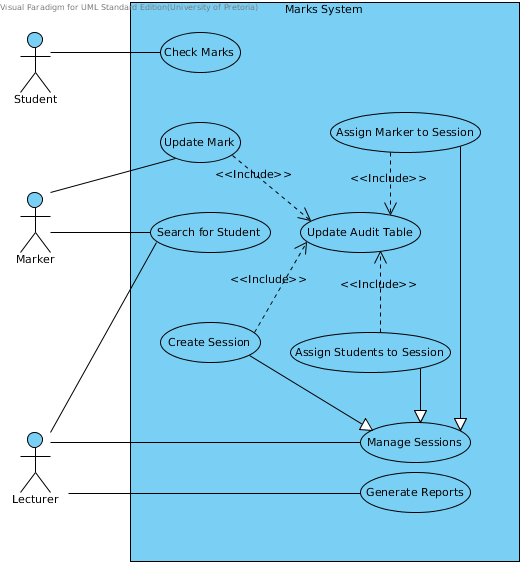
\includegraphics[width=\linewidth]{High_Level_Use_Case_Diagram.png}

\subsection{Required Functionality}
nvanrooyen will do use case diagrams. Will be done by Tuesday.
\section{Risks and open issues}
\begin{itemize}
\item Not all markers, lectures and students will have mobile devices that run andriod.
\item 
\end{itemize}
\section{Glossary}
\begin{itemize}
\item UML - Unified Modeling Language
\item LDAP - Lightweight Directory Access Protocol
\item CSV - Comma-separated values
\item Andriod - Is an operating system based on the Linux kernel
\item Practical - A booked session where practicals are displayed and question can be asked about the weeks practical
\item Authentication - Grant access if details are legitimate
\item Lecture - A person who gives lectures and manages the course
\item Marker - Person that evaluates the practicals
\item Normal distribution - Is a very commonly occurring continuous probability distribution.
\end{itemize}
\end{document}
